\section{光滑曲线的第二个要求}

上一章讨论了光滑的第一个要求——不断,本章讨论我们定义光滑的第二个要求——不折。
如下曲线,在$x_0$处折了。

\begin{figure}[h]
\centering
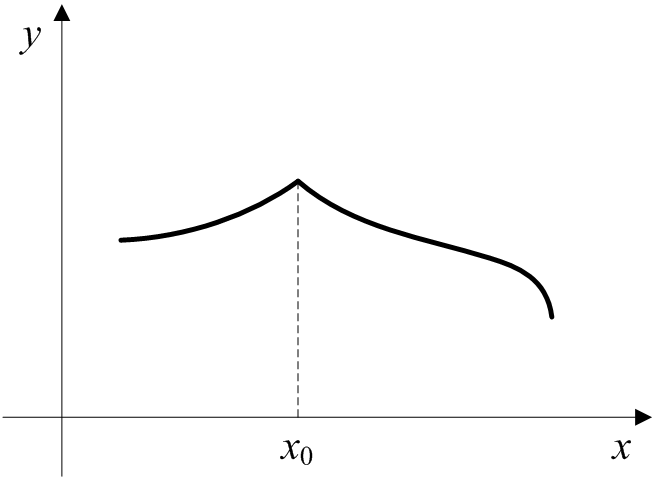
\includegraphics[height=4cm]{2.1.png}
\end{figure}




